\documentclass[12pt,a4paper]{article}
\usepackage[utf8]{inputenc}
\usepackage{hyperref}
\usepackage{amsmath}
\usepackage{amsfonts}
\usepackage{amssymb}
\usepackage{indentfirst}
\usepackage{graphicx}
\usepackage{wrapfig}
\usepackage{color}
\usepackage{float}
\usepackage{listings}
\lstset{ %
language=C,                     % choose the language of the code
basicstyle=\footnotesize,       % the size of the fonts that are used for the code
numbers=left,                   % where to put the line-numbers
numberstyle=\footnotesize,      % the size of the fonts that are used for the line-numbers
stepnumber=1,                   % the step between two line-numbers. If it is 1 each line will be numbered
numbersep=5pt,                  % how far the line-numbers are from the code
backgroundcolor=\color{white},  % choose the background color. You must add \usepackage{color}
showspaces=false,               % show spaces adding particular underscores
showstringspaces=false,         % underline spaces within strings
showtabs=false,                 % show tabs within strings adding particular underscores
frame=single,                   % adds a frame around the code
tabsize=2,                      % sets default tabsize to 2 spaces
captionpos=b,                   % sets the caption-position to bottom
breaklines=true,                % sets automatic line breaking
breakatwhitespace=false,        % sets if automatic breaks should only happen at whitespace
escapeinside={\%}            % if you want to add a comment within your code
}



\title{EP 1 - Programação Concorrente}
\author{Alberto Bueno Júnior - Nº USP: 6514202\\Daniel Francisco Reverbel - Nº USP: 4512210\\Felipe Simionato Solferini - Nº USP: 6431304}
\date{Maio de 2011}

 
\begin{document}
\maketitle
\pagebreak
\tableofcontents
\pagebreak

\section{Introdução ao trabalho}
Este é um trabalho feito para a disciplina "MAC0438 - Programação Concorrente", ministrada, em 2011, pelo professor Daniel Macêdo Batista (\url{http://www.ime.usp.br/~batista}). 
Esta disciplina é oferecida aos alunos de graduação em Ciência da Computação do Instituto de Matemática e Estatística (IME - \url{http://www.ime.usp.br}) da Universidade de São Paulo (USP - \url{http://www.usp.br}).

\section{Problema}
O programa deste trabalho simula um analisador de pacotes de rede. Este dispositivo recebe pacotes e os copia para um disco rígido interno, para análise posterior. A parte deste programa é, na verdade, lidar com os pacotes que chegam ao dispositivo e simular uma cópia para o disco rígido. A entrada do programa é \textbf{M} e \textbf{N}. \textbf{M} representa o número de pacotes que irão chegar e devem ser copiados. \textbf{N} representa o número de processos copiadores que rodam concorrentemente.

\pagebreak
\section{Código}
ep1.c:
\begin{lstlisting}
/* Alberto Bueno Junior
 * Felipe Solferini
 * Daniel Reverbel
 * 
 * Compilando:  gcc -Wall -pthread ep1.c -o ep1
 * Rodando: ./ep1 <m> <n> [s]
 */

#include <stdio.h>
#include <stdlib.h>
#include <pthread.h> /* Para trabalhar com threads */
#include <sys/time.h>
#include <unistd.h>

#define COPY_RATE 0.75 /* bytes / ms */
#define MIN_CHEGADA 250 /* ms */
#define MAX_CHEGADA 1000 /* ms */
#define MAX_TAMANHO 1500 /* bytes */
#define CONV 10

struct pacote {
	int t_chegada;
	int tamanho;
};
typedef struct pacote* pacote_pointer;

struct node {
	pacote_pointer pacote;
	struct node* next;
};
typedef struct node * node_pointer;

struct dados {
	int pac_copiados;
	int b_copiados;
	double ociosidade_total;
	double tempo_total;
};
typedef struct dados *copiador_dados;

/* Variaveis globais */
int senha;
int copiados;
node_pointer head;
node_pointer tail;
copiador_dados *cop_dados;
static pthread_mutex_t cs_mutex = PTHREAD_MUTEX_INITIALIZER;

/* Cria novo no, para depois ser colocado na fila */
node_pointer novo_node() {
	node_pointer novo;
	novo = (node_pointer) malloc(sizeof(* novo) );
	if (novo == NULL) {
		perror("Malloc ERROR no novo");
		exit(1);
	}
	novo->pacote = (pacote_pointer) malloc(sizeof(*novo->pacote) );
	novo->pacote->t_chegada = MIN_CHEGADA + (rand() % (MAX_CHEGADA - MIN_CHEGADA) );
	novo->pacote->tamanho = 1 + (rand() % MAX_TAMANHO);
	novo->next = NULL;
	return novo;
}
/* Verifica se a fila esta vazia */
int fila_vazia() {
	pthread_mutex_lock( &cs_mutex );
	if (head->next == NULL) {
		pthread_mutex_unlock( &cs_mutex );
		return 1;
	}
	else {
		pthread_mutex_unlock( &cs_mutex );
		return 0;
	}
}

/* Funcao que sera usada nas threads 'copiador' */
void * copiador (int *n) {
	struct timeval t_antes, t_depois, t_final;
	double delta;
	node_pointer prox;
	float espera;
	while(1) {
		gettimeofday(&t_antes, NULL);
		while(fila_vazia()) {
			usleep(MIN_CHEGADA * 500);
		}
		gettimeofday(&t_depois, NULL);
		delta = (t_depois.tv_sec - t_antes.tv_sec) + (t_depois.tv_usec - t_antes.tv_usec) / 1000000; /* s */
		/* Inicio da secao critica */
		pthread_mutex_lock( &cs_mutex );
		prox = head->next;
		if (prox == NULL) {
			pthread_mutex_unlock( &cs_mutex );
			continue;
		}
		head->next = prox->next;
		if (prox == tail) {
			tail = head;
		}
		pthread_mutex_unlock( &cs_mutex );
		/* Final da secao critica */
		espera = prox->pacote->tamanho / (float) COPY_RATE;
		usleep((espera * 1000) / CONV);
		cop_dados[*n]->b_copiados += prox->pacote->tamanho;
		cop_dados[*n]->pac_copiados += 1;
		cop_dados[*n]->ociosidade_total += delta;
		gettimeofday(&t_final, NULL);
		delta = (t_final.tv_sec - t_antes.tv_sec) + (t_final.tv_usec - t_antes.tv_usec) / 1000000; /* s */
		cop_dados[*n]->tempo_total += delta;
		copiados++;
	}

	return NULL;
}

/* Funcao que sera usada nas threads 'pacote' */
void * pacote (int *n) {
	node_pointer novo;

	/* Criando pacote */
	novo = novo_node();
	/* Espera a sua vez */
	while (senha != *n) {
		usleep((MIN_CHEGADA * 100) / CONV);
	}
	/* Rodando o processo */
	usleep((novo->pacote->t_chegada * 1000) / CONV);
	/* Inicio da secao critica */
	pthread_mutex_lock( &cs_mutex );
	novo->next = NULL;
	tail->next = novo;
	tail = novo;
	senha++;
	pthread_mutex_unlock( &cs_mutex );
	/* Final da secao critica */
	return NULL;
}

int main (int argc, char *argv[]) {
	/* ====== Declaracoes ====== */
	int i, m, n, seed, script_out;
	pthread_t * ids_pacotes; /* Guardam os ids das threads */
	pthread_t * ids_copiadores;
	int * arg; /* Vetor com os argumentos passados para cada thread */
	/* m = quantidade total de pacotes a serem lidos */
	/* n = quantidade de pacotes que podem ser copiados simultaneamente */

	/* ====== Inicializacoes ====== */
	if (argc == 3) {
		m = atoi(argv[1]);
		n = atoi(argv[2]);
		script_out = 0;
	}
	else {
		if (argc == 4) {
			script_out = 1;
			m = atoi(argv[1]);
			n = atoi(argv[2]);
		}
		else {
			script_out = 0;
			printf("Entrada incorreta!\n");
			return -1;
		}
	}
	seed = time(NULL);
	srand(seed);
	senha = 0;
	head = (node_pointer) malloc(sizeof(*head) );
	if (head == NULL) {
		perror("Malloc ERROR no HEAD");
		exit(1);
	}
	head->pacote = NULL;
	head->next = NULL;
	tail = head;
	cop_dados = (copiador_dados *) malloc(n * sizeof(copiador_dados) );
	if (cop_dados == NULL) {
		perror("Malloc ERROR no cop_dados");
		exit(1);
	}
	for (i = 0; i < n; i++) {
		cop_dados[i] = (copiador_dados) malloc(sizeof(struct dados) );
		if (cop_dados[i] == NULL) {
			perror("Malloc ERROR no cop_dados[i]");
			exit(1);
		}
		cop_dados[i]->b_copiados = 0;
		cop_dados[i]->ociosidade_total = 0;
		cop_dados[i]->tempo_total = 0;
		cop_dados[i]->pac_copiados = 0;
	}

	/* ====== Malloca os vetores ====== */
	ids_pacotes = (pthread_t *) malloc(m * sizeof(pthread_t));
	if (ids_pacotes == NULL) {
		perror("Malloc ERROR no ids_pacotes");
		exit(1);
	}
	if (!ids_pacotes) {
		fprintf(stderr,"Erro no malloc do pthread_t\n");
		return(1);
	}
	ids_copiadores = (pthread_t *) malloc(n * sizeof(pthread_t));
	if (!ids_copiadores) {
		fprintf(stderr,"Erro no malloc do pthread_t\n");
		return(1);
	}
	arg = (int *) malloc(m * sizeof(int) );
	if (!arg) {
		free(ids_pacotes);
		free(ids_copiadores);
		fprintf(stderr,"Erro no malloc do vetor\n");
		return(1);
	}

	/* ====== Inicializa os copiadores ====== */
	for (i = 0; i < n; i++) {
		arg[i] = i;
		if (pthread_create(&(ids_copiadores[i]),NULL,(void *)copiador,(void *)&(arg[i]))) {
			fprintf(stderr,"Erro no pthread_create\n");
			free(ids_pacotes);
			free(ids_copiadores);
			free(arg);
			return(2);
		}
	}
	for (i = 0; i < m; i++) {
		arg[i] = i;
		if (pthread_create(&(ids_pacotes[i]),NULL,(void *)pacote,(void *)&(arg[i]))) {
			fprintf(stderr,"Erro no pthread_create\n");
			free(ids_pacotes);
			free(ids_copiadores);
			free(arg);
			return(2);
		}
	}
	/* ====== LOOP PRINCIPAL ====== */
	while(copiados < m) {
		usleep(1000);
	}

	for (i = 0; i < n; i++) {
		if (script_out) {
			printf("%d %d %d %.2f %.2f\n", i + 1, cop_dados[i]->pac_copiados, cop_dados[i]->b_copiados, cop_dados[i]->ociosidade_total, cop_dados[i]->tempo_total);
		}
		else {
			printf("C%d: %d pacotes, %d bytes, %.2f s (total = %.2f s)\n", i + 1, cop_dados[i]->pac_copiados, cop_dados[i]->b_copiados, cop_dados[i]->ociosidade_total, cop_dados[i]->tempo_total);
		}
	}

	free(ids_copiadores);
	free(ids_pacotes);
	return(0);
}

\end{lstlisting}
\pagebreak

\section{Sobre os testes}

Foram relalizados testes com o seguinte conjunto de entradas:
\\
\begin{itemize}
	\item \textbf{M} = 10 e \textbf{N} = 1
	\item \textbf{M} = 100 e \textbf{N} = 1
	\item \textbf{M} = 1000 e \textbf{N} = 1
	\item \textbf{M} = 1000 e \textbf{N} = 10
	\item \textbf{M} = 1000 e \textbf{N} = 100
	\item \textbf{M} = 1000 e \textbf{N} = 1000
	\item \textbf{M} = 1000 e \textbf{N} = 10000
\end{itemize}

\pagebreak
Todos os testes foram automatizados com os scrips escritos na lingaguem \textit{Perl}. Além disso, cada teste foi realizado 30 vezes. 
Com os dados obtidos de cada um deles, montamos três tipos diferentes de gráfico:

\begin{itemize}
	\item \textbf{Média de cópias por copiador:} No eixo X, os copiadores. No eixo Y, a média de cópias realizada por cada copiador.
	\item \textbf{Média de Bytes copiados:} No eixo X, os copiadores. No eixo Y, a média do número de Bytes copiados por cada copiador.
	\item \textbf{Média de ociosidade:} No eixo X, os copiadores. No eixo Y, a média do tempo de ociosidade de cada copiador (em vermelho) e a média do tempo total de
	execução da thread representada pelo copiador (em verde).
\end{itemize}

\subsection{Máquina utilizada}
Os testes foram realizados em um Laptop Dell Inspiron - Intel Core 2 Duo; 4 GB de memória.

\pagebreak
\section{Testes}
\subsection{Teste 1 - M = 10, N = 1}
\begin{center}
\begin{figure}[H]
    \center
    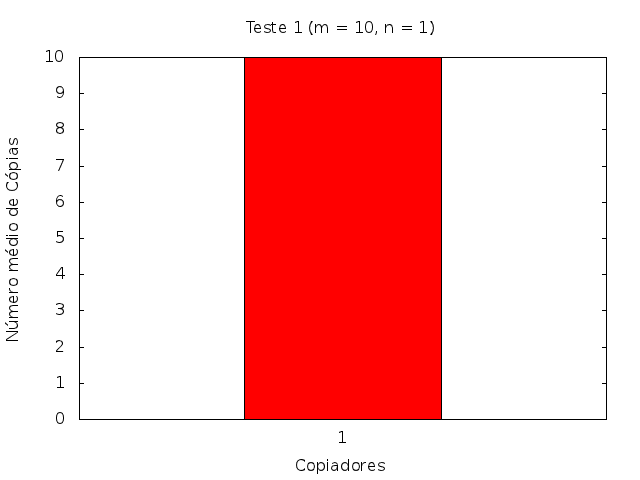
\includegraphics[scale=0.5]{imagens/grafico_copias1.png}
    \label{teste1_copias}
\end{figure}
\end{center}

MAX CÓPIAS = 10
\\
MIN CÓPIAS = 0

\begin{center}
\begin{figure}[H]
    \center
    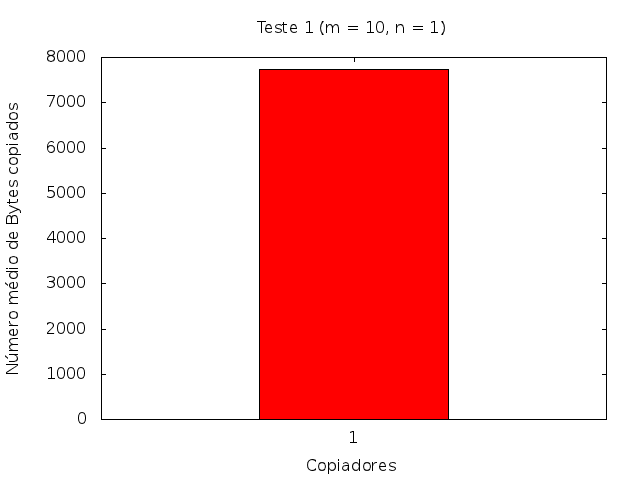
\includegraphics[scale=0.5]{imagens/grafico_bytes1.png}
    \label{teste1_bytes}
\end{figure}
\end{center}

\begin{center}
\begin{figure}[H]
    \center
    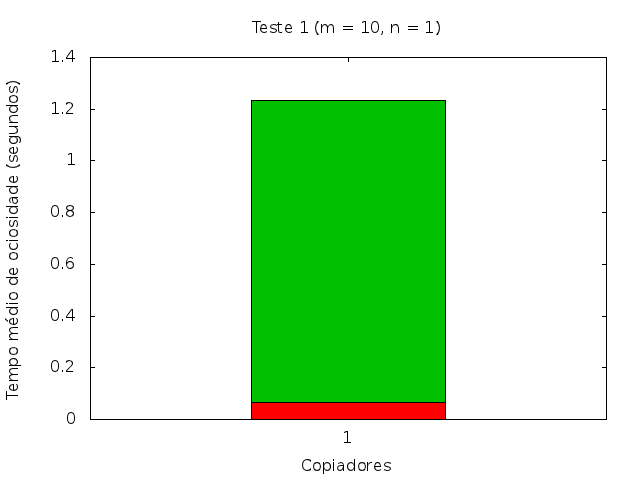
\includegraphics[scale=0.5]{imagens/grafico_ociosidade1.png}
    \label{teste1_ociosidade}
\end{figure}
\end{center}

\pagebreak
\subsection{Teste 2 - M = 100, N = 1}
\begin{center}
\begin{figure}[H]
    \center
    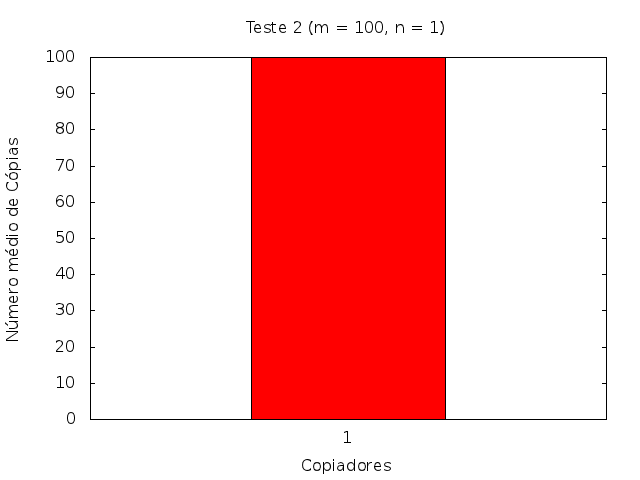
\includegraphics[scale=0.5]{imagens/grafico_copias2.png}
    \label{teste2_copias}
\end{figure}
\end{center}

MAX CÓPIAS = 100
\\
MIN CÓPIAS = 0

\begin{center}
\begin{figure}[H]
    \center
    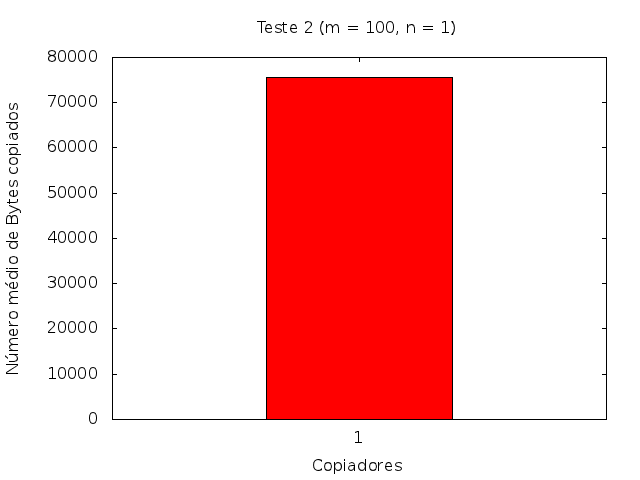
\includegraphics[scale=0.5]{imagens/grafico_bytes2.png}
    \label{teste2_bytes}
\end{figure}
\end{center}

\begin{center}
\begin{figure}[H]
    \center
    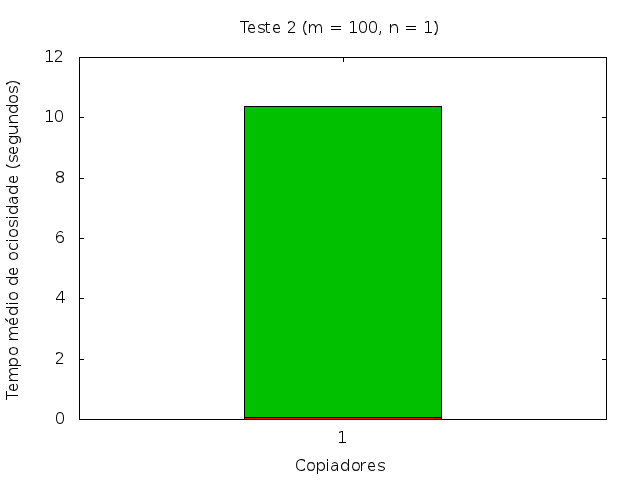
\includegraphics[scale=0.5]{imagens/grafico_ociosidade2.png}
    \label{teste2_ociosidade}
\end{figure}
\end{center}

\pagebreak
\subsection{Teste 3 - M = 1000, N = 1}
\begin{center}
\begin{figure}[H]
    \center
    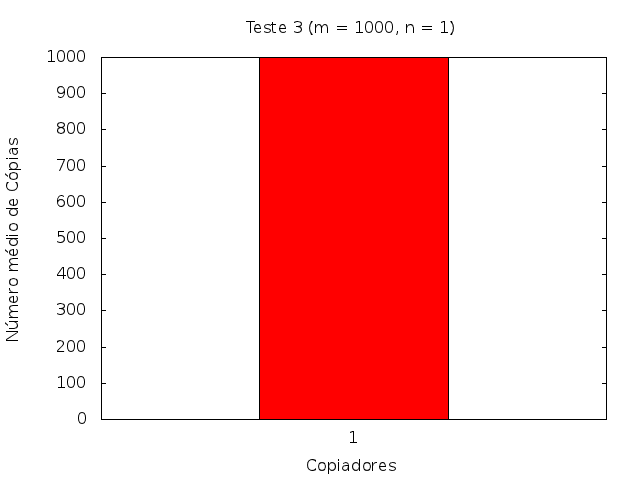
\includegraphics[scale=0.5]{imagens/grafico_copias3.png}
    \label{teste3_copias}
\end{figure}
\end{center}

MAX CÓPIAS = 1000
\\
MIN CÓPIAS = 0

\begin{center}
\begin{figure}[H]
    \center
    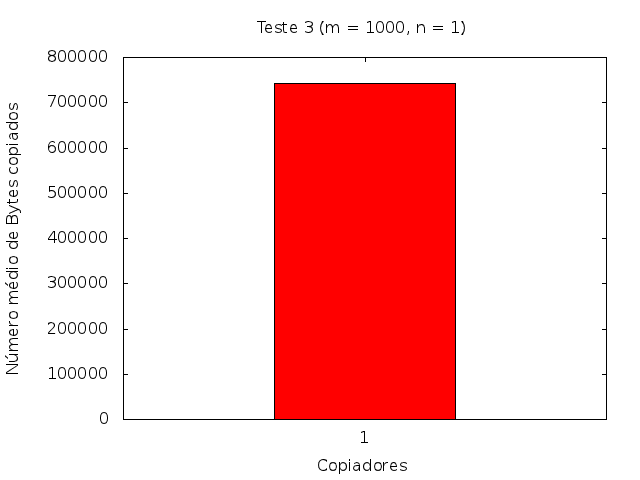
\includegraphics[scale=0.5]{imagens/grafico_bytes3.png}
    \label{teste3_bytes}
\end{figure}

\end{center}
\begin{center}
\begin{figure}[H]
    \center
    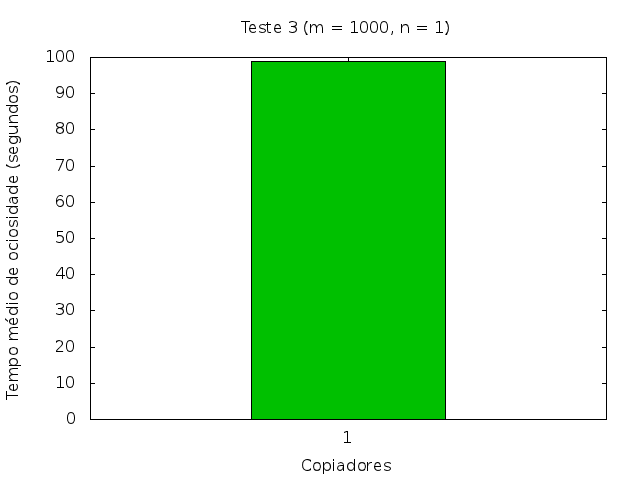
\includegraphics[scale=0.5]{imagens/grafico_ociosidade3.png}
    \label{teste3_ociosidade}
\end{figure}
\end{center}

\pagebreak
\subsection{Teste 4 - M = 1000, N = 10}
\begin{center}
\begin{figure}[H]
    \center
    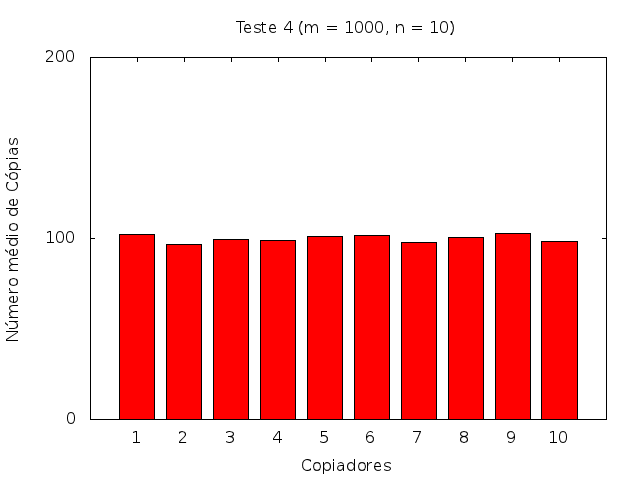
\includegraphics[scale=0.5]{imagens/grafico_copias4.png}
    \label{teste4_copias}
\end{figure}
\end{center}

MAX CÓPIAS = 127
\\
MIN CÓPIAS = 0

\begin{center}
\begin{figure}[H]
    \center
    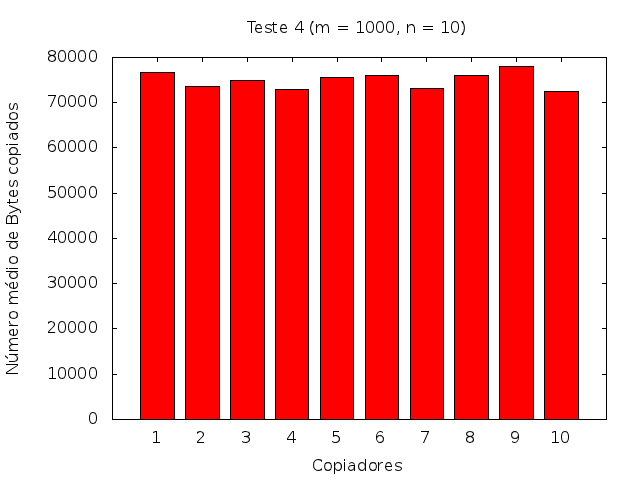
\includegraphics[scale=0.5]{imagens/grafico_bytes4.png}
    \label{teste4_bytes}
\end{figure}
\end{center}

\begin{center}
\begin{figure}[H]
    \center
    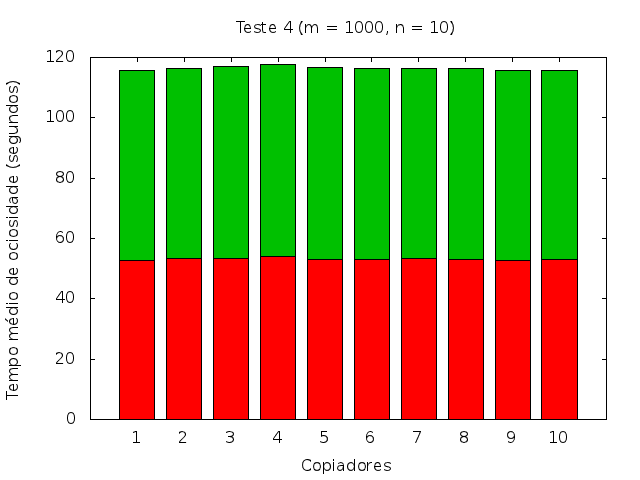
\includegraphics[scale=0.5]{imagens/grafico_ociosidade4.png}
    \label{teste4_ociosidade}
\end{figure}
\end{center}

\pagebreak
\subsection{Teste 5 - M = 1000, N = 100}
\begin{center}
\begin{figure}[H]
    \center
    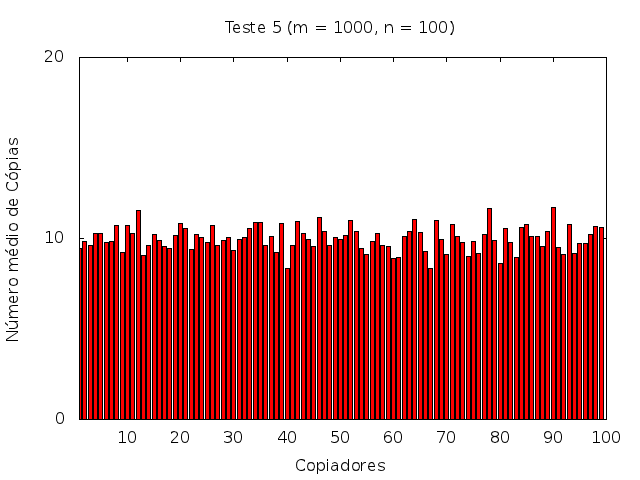
\includegraphics[scale=0.5]{imagens/grafico_copias5.png}
    \label{teste5_copias}
\end{figure}
\end{center}

MAX CÓPIAS = 23
\\
MIN CÓPIAS = 0

\begin{center}
\begin{figure}[H]
    \center
    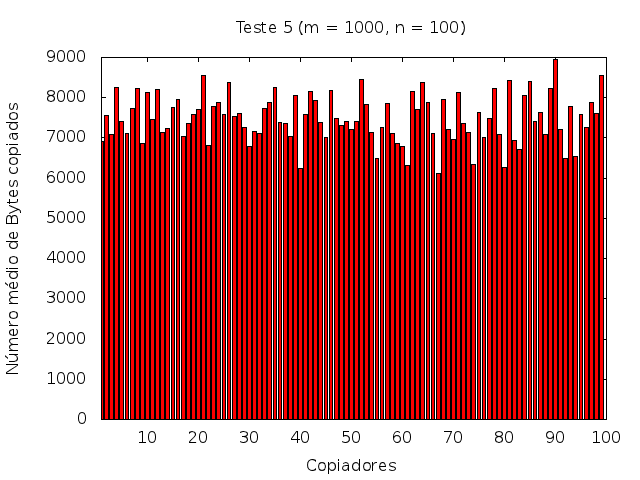
\includegraphics[scale=0.5]{imagens/grafico_bytes5.png}
    \label{teste5_bytes}
\end{figure}
\end{center}

\begin{center}
\begin{figure}[H]
    \center
    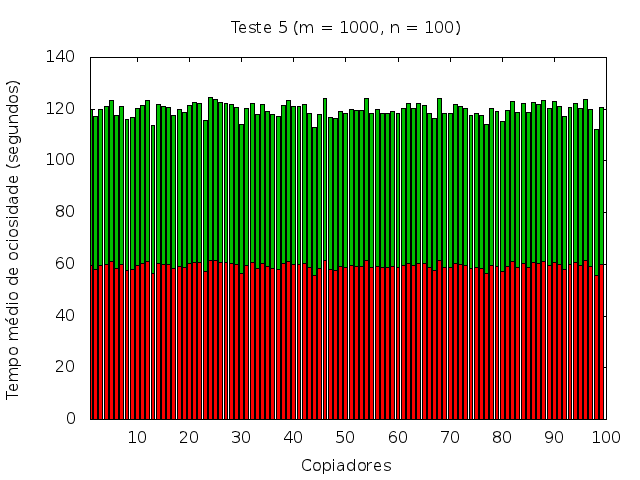
\includegraphics[scale=0.5]{imagens/grafico_ociosidade5.png}
    \label{teste5_ociosidade}
\end{figure}
\end{center}

\pagebreak
\subsection{Teste 6 - M = 1000, N = 1000}
\begin{center}
\begin{figure}[H]
    \center
    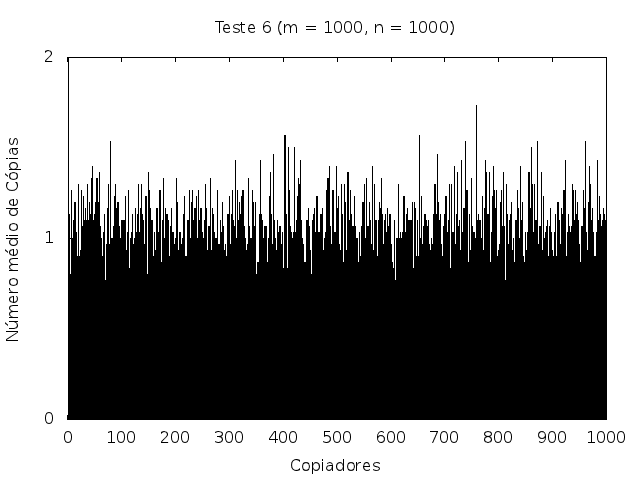
\includegraphics[scale=0.5]{imagens/grafico_copias6.png}
    \label{teste6_copias}
\end{figure}
\end{center}

MAX CÓPIAS = 7
\\
MIN CÓPIAS = 0

\begin{center}
\begin{figure}[H]
    \center
    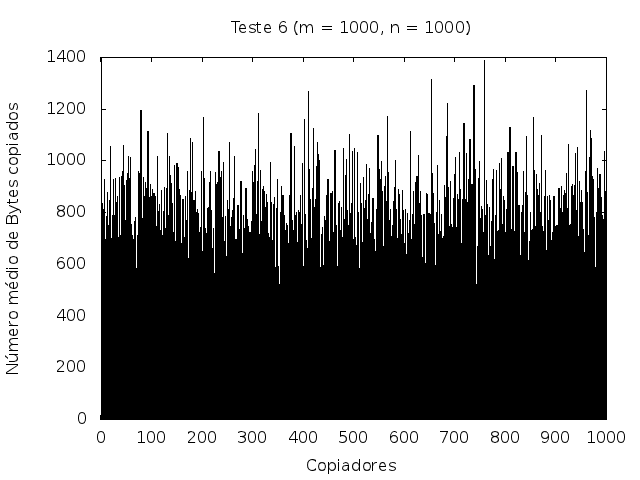
\includegraphics[scale=0.5]{imagens/grafico_bytes6.png}
    \label{teste6_bytes}
\end{figure}
\end{center}

\begin{center}
\begin{figure}[H]
    \center
    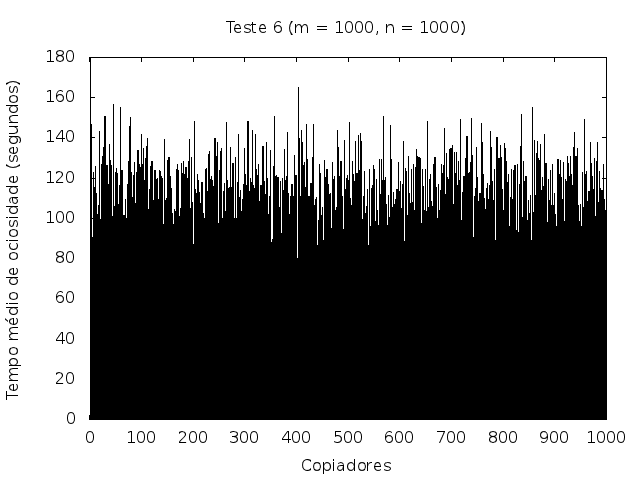
\includegraphics[scale=0.5]{imagens/grafico_ociosidade6.png}
    \label{teste6_ociosidade}
\end{figure}
\end{center}

\pagebreak
\subsection{Teste 7 - M = 1000, N = 10000}
\begin{center}
\begin{figure}[H]
    \center
    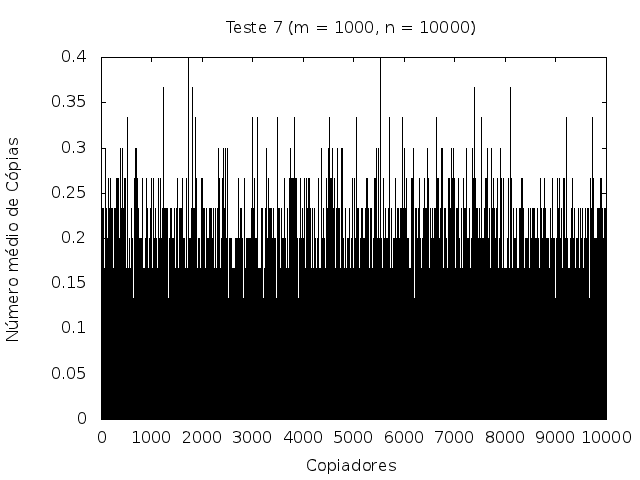
\includegraphics[scale=0.5]{imagens/grafico_copias7.png}
    \label{teste7_copias}
\end{figure}
\end{center}

MAX CÓPIAS = 5
\\
MIN CÓPIAS = 0

\begin{center}
\begin{figure}[H]
    \center
    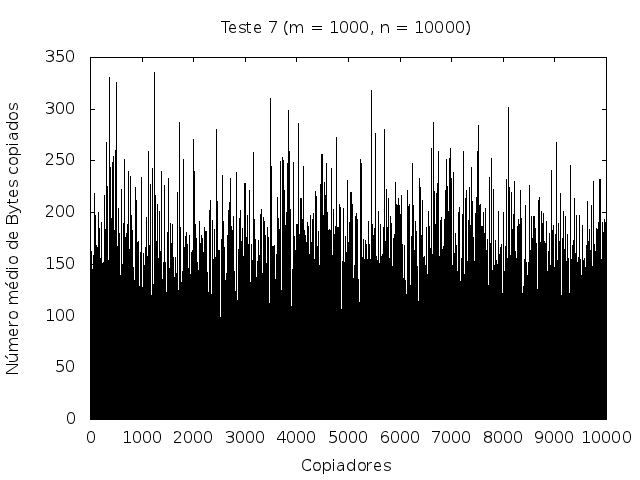
\includegraphics[scale=0.5]{imagens/grafico_bytes7.png}
    \label{teste7_bytes}
\end{figure}
\end{center}

\begin{center}
\begin{figure}[H]
    \center
    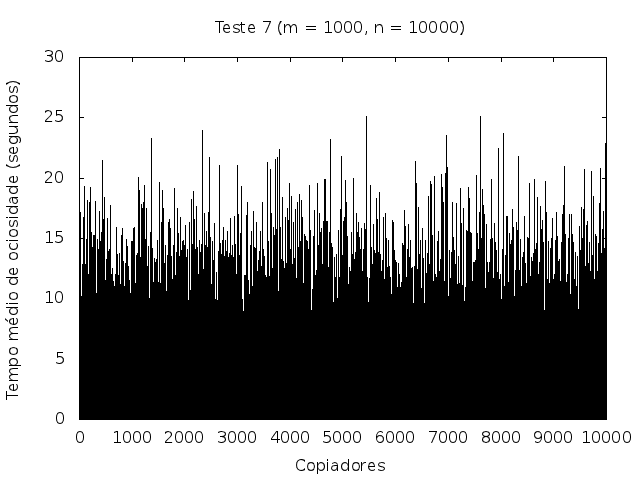
\includegraphics[scale=0.5]{imagens/grafico_ociosidade7.png}
    \label{teste7_ociosidade}
\end{figure}
\end{center}

\pagebreak
\section{Conclusões}
Durante a etapa de codificação do programa, percebemos que foi necessário
adicionar o comando "usleep" nos processos rodando em paralelo. Isso fazia com que 
os processos não sobrecarregassem a CPU do computador com condicionais desnecessárias.
\\
Procuramos estabelecer um valor de \textit{sleep} adequado para não prejudicar a eficiência 
do algoritmo e gerar ociosidade articial e indesejada.
\\
Ao realizar os testes, percebemos também que era necessário limitar o tamanho
da pilha de cada thread, caso contrário não era possível alocar memória para todas elas. 
Para tanto, utilizamos o comando do Linux \textit{ulimit}.

\end{document}
